\documentclass{beamer}
\usepackage{tcolorbox}
\ProvidesPackage{notation}
\RequirePackage{tcolorbox}
\RequirePackage{bm}
\usepackage{amsmath}
\usepackage{tikz}
\usepackage{pgfplots}
\usepackage{adjustbox}
\usepackage{calculator}
\usetikzlibrary{calc}

\pgfplotsset{compat=1.14}

% Draw vector and corresponding unitvector
\newcommand{\vecuvec}[2] %start point, end point (of vector)
{   \VECTORSUB(#2)(#1)(\sola,\solb,\solc)
	\UNITVECTOR(\sola, \solb, \solc)(\sola,\solb,\solc)
	%arrow in blue
	\draw[->,thick,blue] (#1) -- (#2); 
	%corresponding unit-vector in red:
	\edef\temp{\noexpand\draw[->, thick,red] (#1) -- ($(#1)+(\sola,\solb,\solc)$);}
	\temp
}


%\beamerdefaultoverlayspecification{<+->}
\newcommand{\data}{\mathcal{D}}

\DeclareMathOperator*{\argmin}{arg\,min}

\newcommand\Item[1][]{%
	\ifx\relax#1\relax  \item \else \item[#1] \fi
	\abovedisplayskip=0pt\abovedisplayshortskip=0pt~\vspace*{-\baselineskip}}


\usetheme{metropolis}           % Use metropolis theme


\title{Geometric Regression}
\date{\today}
\author{Nipun Batra}
\institute{IIT Gandhinagar}
\begin{document}
	\maketitle
	
	
	\begin{frame}{Linear Combination of Vectors}
		Let $v_{1},v_{2},v_{3},\dots,v_{i}$ be vectors in  ${\rm I\!R}^{D}$, where $D$ denotes the dimensions. A linear combination of $v_{1},v_{2},v_{3},\dots,v_{i}$ is of the following form
		
		\begin{equation*}
			\alpha_{1}x_{1}+			\alpha_{2}x_{2}+			\alpha_{3}x_{3}+
			\dots+\alpha_{i}x_{i}
		\end{equation*}
		
		where $\alpha_{1},\alpha_{2},\alpha_{3},\dots,\alpha_{i} \in {\rm I\!R}$
		
	\end{frame}

\begin{frame}{Span of vectors}
		Let $v_{1},v_{2},\dots,v_{i}$ be vectors in  ${\rm I\!R}^{D}$, with $D$ dimensions. \\
		The span of  $v_{1},v_{2},\dots,v_{i}$ is denoted by SPAN\{$v_{1},v_{2},\dots,v_{i} $\}
		
		\begin{equation*}
	    \{	\alpha_{1}x_{1}+			\alpha_{2}x_{2}+
		\dots+\alpha_{i}x_{i} \hspace{1em}\vert \hspace{1em}  \alpha_{1},\alpha_{2},\dots,\alpha_{i} \in {\rm I\!R}\}
		\end{equation*}
		
		The above denotes the span of the vectors $v_{1},v_{2},\dots,v_{i}$.  It is the set of all vectors that can be gengerated by linear combinations of $v_{1},v_{2},\dots,v_{i}$.
\end{frame}


\begin{frame}{Subspace}
	A subset $S$ $\in {\rm I\!R}$ is called a subspace if  
	\begin{itemize}
		\item origin belongs to $S$
		\item if $u,v \in S$, then $u+v \in S$  
		\item if $u \in S$, then $\alpha u \in S$,  $\forall \alpha \in {\rm I\!R}$
	\end{itemize}	
\end{frame}

\begin{frame}{When does a Span become a subspace?}
	Think about it!
\end{frame}


\begin{frame}{}	\begin{columns}
	\pause \begin{column}{0.6\textwidth}
		\begin{adjustbox}{max totalsize={\textwidth},center}
			
			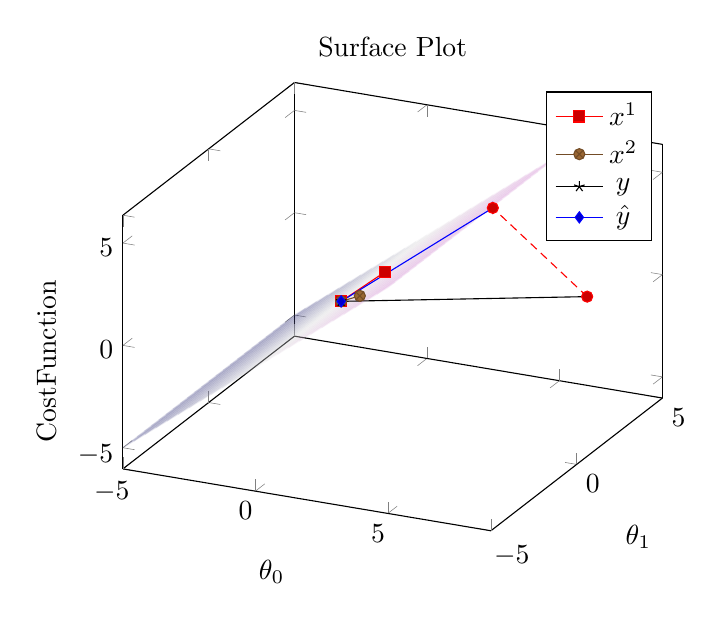
\begin{tikzpicture}
			\begin{axis}[xlabel=$\theta_0$, ylabel=$\theta_1$, zlabel=$\mathrm{Cost Function}$,title={Surface Plot}]
			\addplot3[
			surf,
			colormap/violet,
			opacity=0.1,
			]
			{x};
			\addplot3 coordinates {
				(0, 0, 0)
				(1, 1, 1)
			};
		\addplot3 coordinates {
			(0, 0, 0)
			(2, -2, 2)
		};
	\addplot3 coordinates {
		(0, 0, 0)
		(8.89, 0.61, 1.77)
	};
	\addplot3 coordinates {
	(0, 0, 0)
	(5.33, 0.61, 5.33)
};
	\addplot3 coordinates {
	(8.89, 0.61, 1.77)
	(5.33, 0.61, 5.33)
};
	\legend{{}, $x^1$,$x^2$, $y$, $\hat{y}$}
			\end{axis}
			\end{tikzpicture}
		\end{adjustbox}
		
	\end{column}
\end{columns}
\end{frame}


\begin{frame}
Solution: 2.97, 1.18
\end{frame}

\begin{frame}
\begin{tikzpicture}
\draw[->](0,0) -- (5,0);
\end{tikzpicture}

\begin{tikzpicture}
\draw[<<->>](0,0) -- (5,0);
\end{tikzpicture}


\begin{tikzpicture}
\draw[<<->>, ultra thick, blue](0,0) -- (5,0);
\end{tikzpicture}

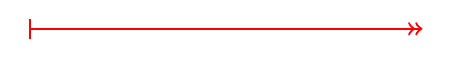
\begin{tikzpicture}
\draw[|->>, thick, red](0,0) -- (5,0);
\end{tikzpicture}



\end{frame}
	


\begin{frame}{Geometric Interpretation of Linear Regression}
	Let $\bar{x_{j}}$ denote the $j^{th}$ column of $X$. \\
	Let $\hat{y}$ be the prediction.
	
	$$
	\hat{y} = w_{1}\bar{x_{1}}+w_{2}\bar{x_{2}}+\dots+w_{D}\bar{x_{D}} = XW
	$$
	
	
	Clearly, $\hat{y} \in $ SPAN\{$\bar{x_{1}},\bar{x_{2}},\dots,\bar{x_{D}}$\} 
	How to choose the best $\hat{y}$?
\end{frame}

\begin{frame}{Geometric Interpretation of Linear Regression}
	We wish to $\hat{y}$ such that 
	$$
		\underset{\hat{y} \in SPAN\{\bar{x_{1}},\bar{x_{2}},\dots,\bar{x_{D}}\} } \argmin \vert \vert y - \hat{y} \vert \vert_{2}
	$$
\end{frame}

%\begin{frame}{Geometric Interpretation of Linear Regression}
%	It is analogus to choosing $\hat_{y}$ such that it is closest to $y$. It is the projection of $y$ onto the column space of $X$.
%	\vspace{2em}\\
%	Hence the residual vector $y - \hat{y}$ will be perpendicular to each of the columns of $X$. 
%\end{frame}



\begin{frame}{Geometric Interpretation of Linear Regression}
	$$
		\bar{x_{i}}(y - \hat{y}) = 0
	$$
	
	$$
		X^{T}(y - XW) = \mathbf{0}
	$$
	
	\begin{tcolorbox}
		$$
			W = (X^{T}X)^{-1}X^{T}y
		$$
	\end{tcolorbox}

	
	
\end{frame}

\begin{frame}
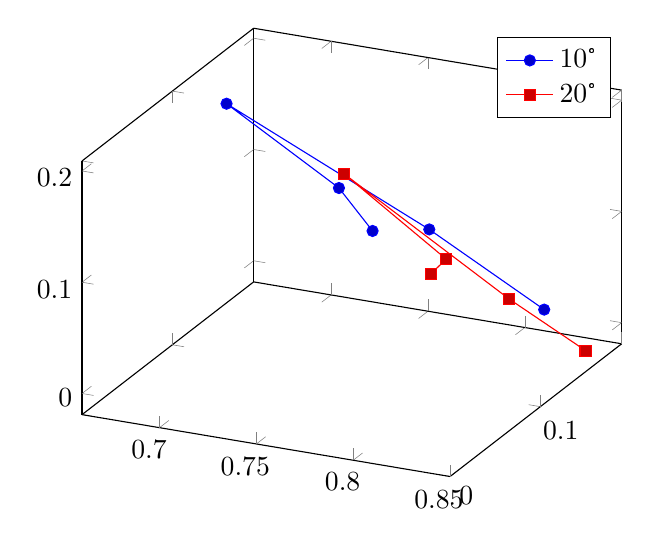
\begin{tikzpicture}
\begin{axis}
\addplot3 coordinates {
	(0.81,	0.19,	0.00)
	(0.76,	0.17,	0.07)
	(0.66,	0.16,	0.16)
	(0.76,	0.07,	0.17)
	(0.81,	0.00,	0.19)
};

\addplot3 coordinates {
	(0.85,	0.15,	0.00)
	(0.82,	0.13,	0.05)
	(0.73,	0.14,	0.13)
	(0.82,	0.06,	0.13)
	(0.84,	0.00,	0.16)
};
\legend{$10$\textdegree, $20$\textdegree}
\end{axis}
\end{tikzpicture}
\end{frame}



\end{document}